% 原文 pp.20--28、2.2節全体。
% 原文 p.20
\hypertarget{srcpage:20}{}\label{srcpage:20}
\subsectionlink{重ね合わせ原理}
重ね合わせ原理は量子力学の核心にあり、古典的な概念からの離脱を最も明瞭に示す特徴の一つである。形式的には、重ね合わせ原理はHilbert空間の線形性に根差している。量子状態はHilbert空間内のベクトルで表されるので、それらのベクトルの線形結合を作れる。重ね合わせ原理によれば、そのようなベクトルの線形結合は、再び新たな量子状態に対応する。これは、ケット$\lvert\psi_n\rangle$が量子状態の集合を表すなら、重ね合わせ
\begin{equation}\lvert\Psi\rangle=\sum_n c_n\lvert\psi_n\rangle\tag{2.1}\end{equation}
もまた、可能で、同じように許される量子状態に対応することを意味する。ここで$c_n$は任意の複素係数である。したがって重ね合わせ原理の平等性により、重ね合わせ状態$\lvert\Psi\rangle$は、成分状態$\lvert\psi_n\rangle$とまったく同様に、系の可能な物理状態に対応する。

たとえばスピン$1/2$の粒子を、二つの状態$\lvert0\rangle$（「上向きスピン」）または$\lvert1\rangle$（「下向きスピン」）の一方に準備できるとしよう。すると重ね合わせ原理は、$\lvert\Psi\rangle=(\lvert0\rangle+\lvert1\rangle)/\sqrt2$も同じように許される量子状態であり、したがって少なくとも原理上は、系をこの重ね合わせ状態にも準備できることを教える。

\subsubsectionlink{重ね合わせの解釈}
重ね合わせ原理がなぜこのような反直観的帰結を持つかを理解するには、量子力学的な重ね合わせを正しく解釈することが不可欠である。このような重ね合わせ状態は、単にその成分の古典的な集団を表すのではない（そのような集団はしばしば真正混合と呼ばれる\cite{ref047,ref048,ref049}）。すなわち、量子系が実際には成分状態$\lvert\psi_n\rangle$の一つだけにあるが、どれであるかを私たちが知らないという状況ではない（これを「素朴な集団解釈」と呼べる）。そうではなく、式(2.1)の各成分$\lvert\psi_n\rangle$が量子状態に同時に存在する。この状況を、それらの成分間にコヒーレンスが存在すると表現する。古典的な場合との違いを明確に強調するため、式(2.1)のような量子力学的重ね合わせは、しばしばコヒーレントな重ね合わせと呼ばれる。本書では、明示的に断らない限り、「重ね合わせ」は常に量子的な、すなわちコヒーレントな重ね合わせを意味する。そのような成分状態の重ね合わせは、個々の系の新しい物理状態を定義するのであって、成分状態の統計分布にすぎないものではない。

% 原文 p.21
\hypertarget{srcpage:21}{}\label{srcpage:21}
重ね合わせを、その成分状態の古典的な集団、すなわち、より根本的に確定された状態の集団と解釈することに反対する、一般的な議論を与えられる。証明は背理法による。状態$\lvert\psi_n\rangle$の重ね合わせ$\lvert\Psi\rangle=\sum_n c_n\lvert\psi_n\rangle$に、実際にそのような集団的見方を与えられると仮定しよう。すると測定によって追加の知識を得て、測定で得た結果と両立する状態からなる部分集団を取り出せる。時間発展はSchrödinger方程式
\begin{equation}i\frac{\mathrm d}{\mathrm dt}\lvert\Psi(t)\rangle=\hat H\lvert\Psi(t)\rangle\tag{2.2}\end{equation}
に従って完全に決定論的であったので、この特定の部分集団を時間を遡って追跡できることになる。その結果、系の初期状態、すなわち測定前の状態を、より完全に指定できる（この過程はしばしば「事後選択」と呼ばれる\cite{ref050}）。これは、その状態が、初めに準備した重ね合わせとは物理的に異なることを意味し、矛盾が生じる。

\subsubsectionlink{重ね合わせの実験的検証}
コヒーレンスの存在を実験で示し、それによって重ね合わせが、その成分状態の集団、すなわち真正混合と実際に異なることを、どう示せばよいだろうか。一般的な方法は二つある。重ね合わせ状態への直接の射影測定を繰り返すことと、干渉実験によって重ね合わせ内のすべての成分の存在を間接的に確認することである。いくつかの単純な例で、この二つの方法を説明しよう。

\paragraph{直接測定}
式(2.1)の形の重ね合わせ状態の存在を確認する最も直接的な方法は、同一に準備された系の集団の各要素について、観測可能量$\hat O=\lvert\Psi\rangle\langle\Psi\rvert$の射影測定を行うことである。各測定で1という結果が得られ、集団が十分大きければ、系は実際に重ね合わせ(2.1)に準備されていたに違いないと結論できる。

そのような測定を実現する装置の例は、Stern--Gerlach装置である（図2.1）。典型的なStern--Gerlach実験は次のように行われる。銀原子を炉で加熱し、コリメート用スリットと、$z$方向に不均一な磁場に通す（簡単のため、他の方向の磁場成分は無視する）。各銀原子は47個の電子を持ち、そのうち46個は球対称な電子雲に収まっている。したがって、47番目の電子のスピンだけが、原子全体の正味の磁気モーメントを与える。よって、比較的大きな質量を持ちながら、その磁気モーメントは単一電子のスピン磁気モーメントに等しい原子を扱うことになる。

% 原文 p.22
\hypertarget{srcpage:22}{}\label{srcpage:22}
\begin{figure}[htbp]\centering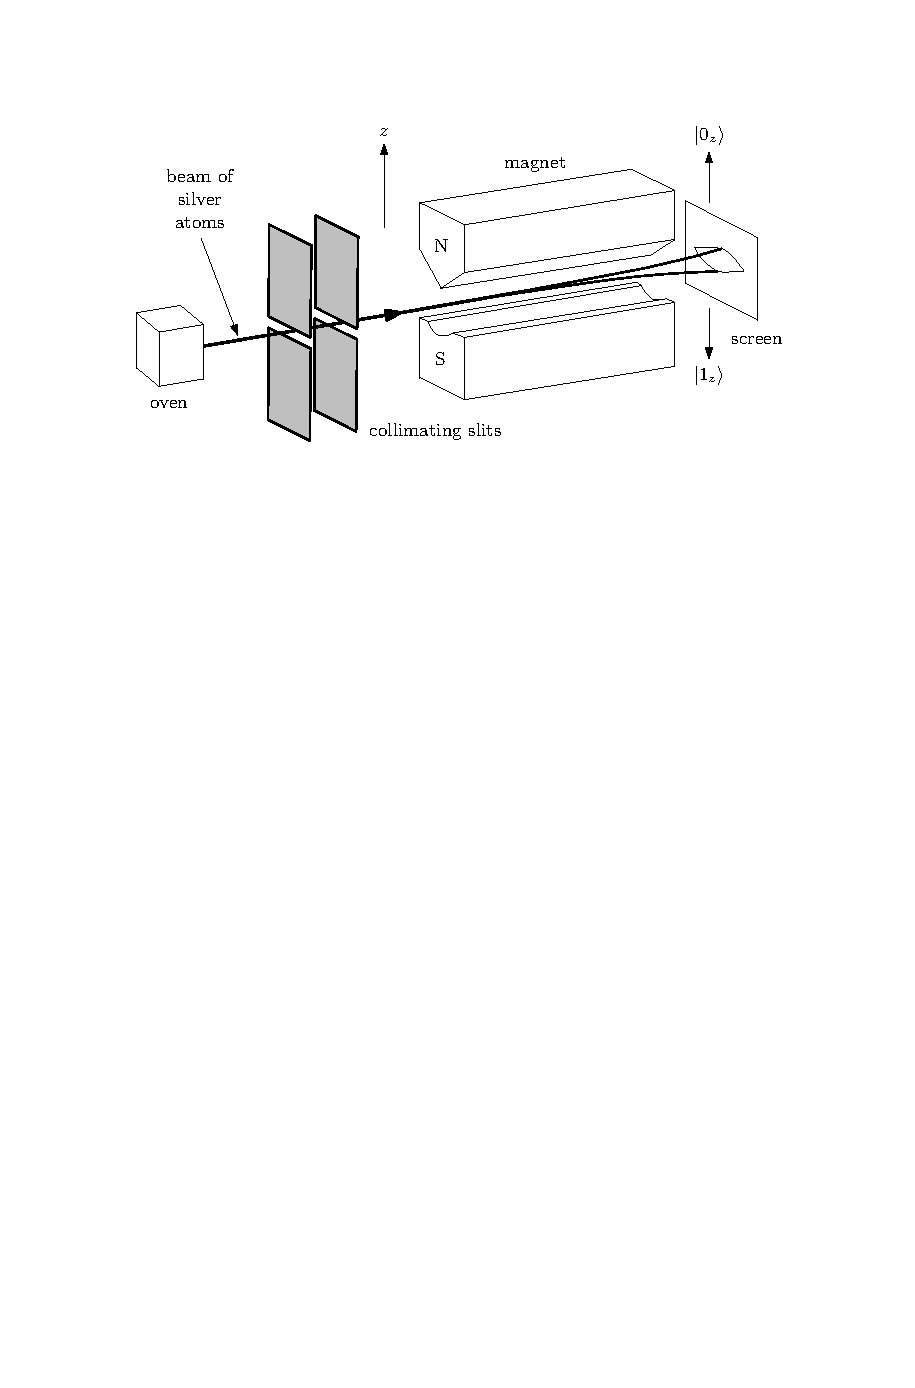
\includegraphics[width=.9\linewidth]{figures/ch02_fig01.pdf}\caption{Stern--Gerlach実験の模式図。単一電子のスピンに等しい磁気モーメントを持つ銀原子が炉から放出され、続いて$z$方向に不均一な磁場を通過する（不均一性は、たとえば磁石の磁極片の形によって生じる）。スピン状態に応じて、原子の経路は二つの可能な軌道に沿って曲げられ、$z$軸方向のスピンの量子化された値を示す。多くの原子が装置を通過すると、検出スクリーン上に二つの明瞭な帯が観測される。}\end{figure}

電子は$z$軸方向に、大きさが等しく向きが反対の二つのスピン値、すなわち「上向き」または「下向き」しか取れないので、銀原子の磁気モーメントには$\pm\mu_z$という二つの可能な値がある。銀原子が不均一な磁場を通過すると、磁気モーメントと磁場の相互作用によって$z$方向の力を受ける。この力は磁気モーメントの値に比例する。したがって、原子内の47番目の電子が$z$軸方向に上向きスピン状態にあるか、下向きスピン状態にあるかに応じて、銀原子の軌道は$+z$方向または$-z$方向に曲がる。これらの状態をそれぞれ$\lvert0_z\rangle$、$\lvert1_z\rangle$と書くことにし、これらはPauliの$z$スピン演算子$\hat\sigma_z$の固有状態である。原子ビームが検出スクリーンに当たると、原子が取りうる二つの異なる軌道に対応して、空間的に分離した二つの斑点が現れる。代わりに、一方の経路に粒子検出器を置けば、特定の原子がその経路を通ったかどうかが分かる。どちらの場合も、この装置は電子スピンの$z$成分の測定に対応する。

% 原文 p.23
\hypertarget{srcpage:23}{}\label{srcpage:23}
入射原子を、電子の$z$軸方向の「上向きスピン」に対応する量子状態、すなわち$z$スピン演算子$\hat\sigma_z$の固有状態$\lvert0_z\rangle$に準備するとしよう。予想どおり、スクリーン上の模様はこの準備を実験的に確認する。すべての原子がスクリーン上部に到達することが分かる。同時に、$\lvert0_z\rangle$は、直交する$x$軸方向の「上向きスピン」と「下向きスピン」の線形結合、$\lvert0_z\rangle=(\lvert0_x\rangle+\lvert1_x\rangle)/\sqrt2$とも等しく書けるので、この実験は、この重ね合わせが準備されたことを確認すると見なせる。もし重ね合わせが状態$\lvert0_x\rangle$と$\lvert1_x\rangle$の古典的な集団を表し、各電子が実際にはそのどちらか一方にあったなら、磁場の不均一性は$z$軸方向だけを向いていて原子ビームを分裂させないため、スクリーン中央に単一の斑点が現れるはずである。もちろん、実験ではそのような振る舞いは観測されない。逆に磁場の向きを90度回転させて$x$方向にすることもできる。この場合、初期状態$\lvert0_z\rangle$に準備したすべての原子について、ビームが50対50に分裂するのが観測される。

したがって重ね合わせ状態$\lvert0_z\rangle=(\lvert0_x\rangle+\lvert1_x\rangle)/\sqrt2$は、成分$\lvert0_x\rangle$と$\lvert1_x\rangle$が同時に存在する、個々の系の物理状態に対応する。それゆえ重ね合わせは、成分$\lvert0_x\rangle$と$\lvert1_x\rangle$の間の干渉縞という形でのみ現れるのではない（下記参照）。むしろ、Stern--Gerlach装置の磁場には、原子の軌道を「確実に予言」できるような向きが必ず存在する\cite{ref010,ref039}。

\paragraph{干渉実験}
Stern--Gerlach装置でのスピン測定の例は、かなり特殊な場合である。重ね合わせ状態に対応する射影観測可能量を直接測定するのは、通常きわめて難しいからである。代わりに、一般に利用できるのは、重ね合わせの成分に対応する特定の基底で測定を行う装置だけである。たとえば、Schrödingerの猫が生きているか死んでいるかを検出できる測定装置、つまり私たち自身の眼は存在する。これは$\{\lvert\text{「生」}\rangle,\lvert\text{「死」}\rangle\}$基底で測定する装置である。しかし、共役な基底$\{(\lvert\text{「生」}\rangle\pm\lvert\text{「死」}\rangle)/\sqrt2\}$で観測可能量を測定することに対応する、明白な手順は存在しない。もちろんこれこそが、Schrödingerの猫の重ね合わせ状態が、あれほど反直観的に見える理由である。普通、私たちにはそのような状態を直接観測する手段、すなわち測定装置、とりわけ人間の感覚がないのである。

この問題のより身近な例として、電子を個々に、すなわち一度に一個ずつ二重スリットに通す、有名な二重スリット実験を考えよう。スリットの位置では、電子は、それぞれスリット1、2を通ることに対応する成分$\lvert\psi_1\rangle$、$\lvert\psi_2\rangle$の重ね合わせ$\lvert\Psi\rangle=(\lvert\psi_1\rangle+\lvert\psi_2\rangle)/\sqrt2$で記述される。この重ね合わせの存在を直接確認するには、状態$\lvert\Psi\rangle$への射影測定が必要である。しかし、波動関数$\Psi(x)\equiv\langle x\vert\Psi\rangle$は、スリットに平行な各平面上で空間的に非局在化している一方、利用できる測定は、スリットの後方における粒子の位置測定だけである。したがって、射影観測可能量$\lvert\Psi\rangle\langle\Psi\rvert$を測定するには、二つの部分波$\psi_1(x)\equiv\langle x\vert\psi_1\rangle$と$\psi_2(x)\equiv\langle x\vert\psi_2\rangle$を、空間内の一点に正確に再集束させる必要がある。明らかに、これは実際上ほとんど不可能である。

% 原文 p.24
\hypertarget{srcpage:24}{}\label{srcpage:24}
このように、重ね合わせの成分状態を測定する手順しか使えない場合には、通常、重ね合わせ内の成分間の干渉効果を示す方法に頼る。基本的な考えは、重ね合わせ状態$\lvert\Psi\rangle=\sum_n c_n\lvert\psi_n\rangle$を定める展開係数$c_n$［式(2.1)］に、空間的または時間的変化を生じさせ、系が成分状態$\lvert\psi_n\rangle$の古典的な集団で記述される場合には、その変化が生じないように実験を設計することである。そのうえで、同一に準備した系の集団について、成分基底$\{\lvert\psi_n\rangle\}$で測定する。$\lvert c_n\rvert^2$は成分状態$\lvert\psi_n\rangle$を見いだす確率を指定するので、その確率が位置または時間に伴って変化することを観測すれば、系は実際に重ね合わせ状態$\lvert\Psi\rangle=\sum_n c_n\lvert\psi_n\rangle$に準備されていたと推論できる。重要な例を二つ挙げよう。

二重スリット実験では、遠方のスクリーン上の密度模様の空間的な変化、すなわちスクリーンの位置での粒子の位置空間密度分布$\varrho(x)$を測定する。よく知られた結果は干渉模様が得られるというものであり、それは、各電子がどちらか一方のスリットを通ると仮定した場合に予想される古典的模様とは、はっきり異なる（図2.2）。密度$\varrho(x)$は、成分状態$\psi_1(x)$と$\psi_2(x)$の古典的分布に対応する、各スリットを個別に通過する寄与の和を記述する波動関数の絶対値二乗の和、すなわち$\varrho(x)\propto\lvert\psi_1(x)\rvert^2+\lvert\psi_2(x)\rvert^2$ではなく、各波動関数の和の絶対値二乗で記述される。
% 原文 p.25
\hypertarget{srcpage:25}{}\label{srcpage:25}
\begin{equation}\begin{split}\varrho(x)&=\frac12\lvert\psi_1(x)+\psi_2(x)\rvert^2\\&=\frac12\lvert\psi_1(x)\rvert^2+\frac12\lvert\psi_2(x)\rvert^2+\operatorname{Re}\{\psi_1(x)\psi_2^*(x)\}.\end{split}\tag{2.3}\end{equation}
最後の項が、スクリーン上の特徴的な干渉模様の原因である。

\begin{figure}[htbp]\centering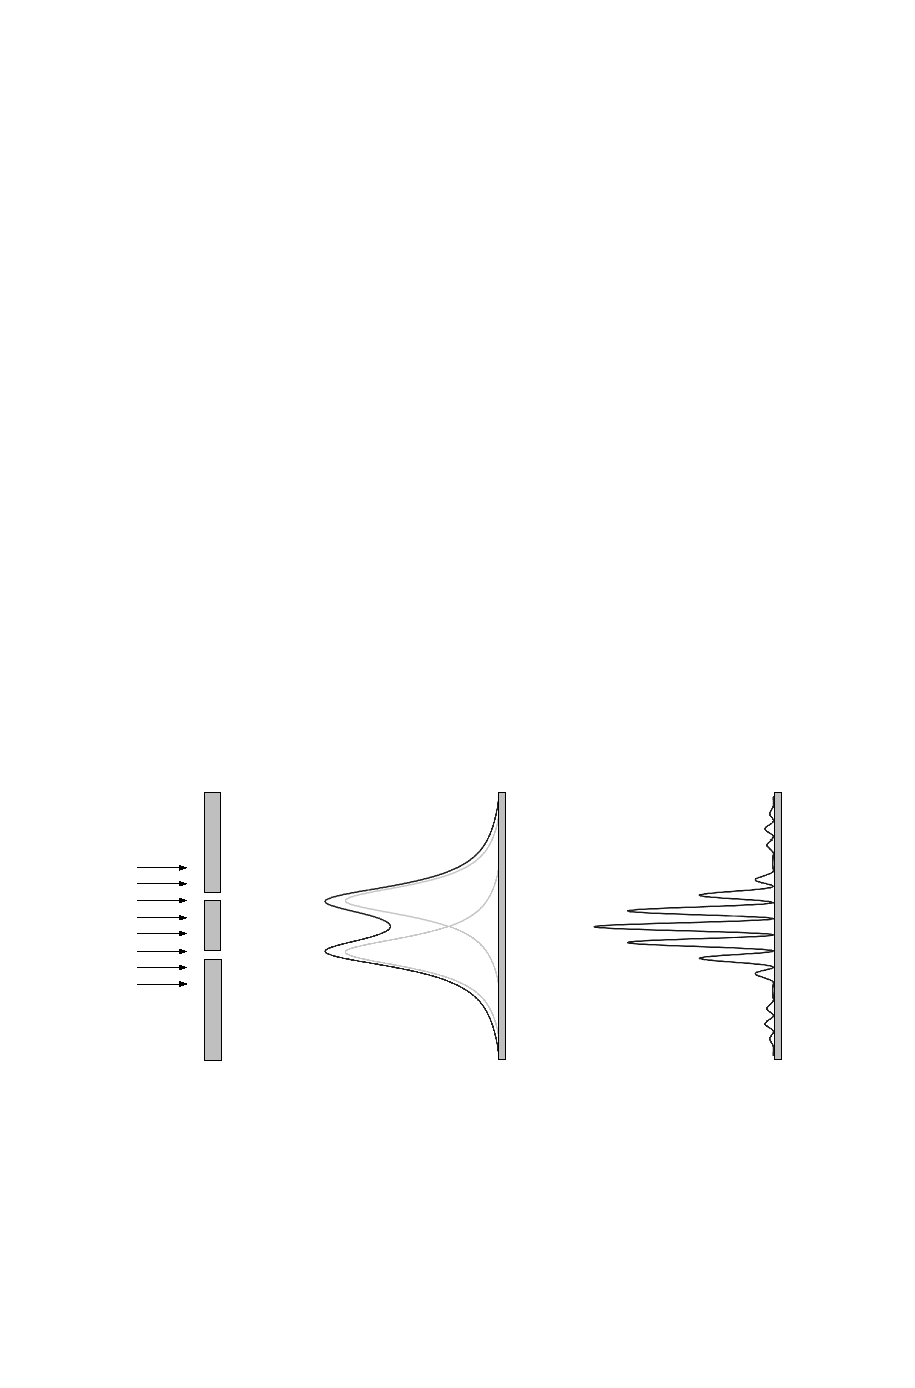
\includegraphics[width=.9\linewidth]{figures/ch02_fig02.pdf}\caption{粒子による二重スリット実験。左：粒子が二重スリットに入射する。中央：遠方の検出スクリーン上に得られる「古典的」密度模様。これは、各スリットからの寄与を単純に足し合わせたものに対応する。右：量子的な設定で得られる干渉模様（包絡線は回折によって変調されている）。}\end{figure}

この実験は、標準的な量子力学の形式の範囲内では\footnote{量子力学には、異なる見方を許す別の定式化も存在する。たとえばBohm力学では、すべての粒子の位置は常に確定しているとされる（8.5節）。したがって各粒子は、二つのスリットの一方を通る確定した軌道を進む。波動関数は依然として両スリットにわたって非局在化しているが、それは粒子が取りうるさまざまな経路を定めるだけである。}、個々の電子を、特定のスリットの通過を記述する一方の波動関数では記述できず、それらの波動関数の重ね合わせ$\Psi(x)=(\psi_1(x)+\psi_2(x))/\sqrt2$によってのみ記述できることを明瞭に示している。形式的には、この知見は、量子状態が実際の確率ではなく確率振幅を表すことによって説明される。つまり重ね合わせ状態は、確率ではなく確率振幅の線形結合を記述し、そのため重ね合わせに対応する確率分布(2.3)に干渉項が生じる。また、任意の時点で装置内に一個の粒子しか存在しないように二重スリット実験を行うことは十分に可能なので（6.2節）、干渉模様を異なる電子間の相互作用のせいにはできないことにも注意しよう。

干渉効果の観測により重ね合わせの存在を間接的に検証する、もう一つの例はRamsey干渉法\cite{ref051}である。今度は空間的変化ではなく時間的変化を用いる。Ramsey干渉法は、二準位系における量子的にコヒーレントなRabi振動の原理に直接基づいており、これは6.1.1節でより詳しく説明する。基底状態$\lvert g\rangle$と励起状態$\lvert e\rangle$で記述される二準位原子があり、その重ね合わせ状態$\lvert\psi\rangle=(\lvert g\rangle+\lvert e\rangle)/\sqrt2$の存在を示したいとしよう。しかし、実験では原子のエネルギー状態しか測定できず、$\{\lvert g\rangle,\lvert e\rangle\}$基底での測定だけが可能で、重ね合わせの直接の射影測定に必要となる共役基底$\{(\lvert g\rangle\pm\lvert e\rangle)/\sqrt2\}$では測定できない。

この場合も、干渉実験を行う方法によって目的を達成できる。まず、観測可能量$\hat O=\lvert g\rangle\langle g\rvert$の射影測定によって原子を基底状態$\lvert g\rangle$に準備する。次に、特定の持続時間のレーザーパルスを加えることによって（詳細は6.1.1節）、この状態をコヒーレントな重ね合わせ
% 原文 p.26
\hypertarget{srcpage:26}{}\label{srcpage:26}
\begin{equation}\lvert\Psi\rangle=\frac1{\sqrt2}(\lvert g\rangle-i\lvert e\rangle)\tag{2.4}\end{equation}
へと変換できる。その後、状態は自由に発展し続ける。
\begin{equation}\lvert\Psi\rangle=\frac1{\sqrt2}\bigl(\lvert g\rangle-ie^{-i\phi(t)}\lvert e\rangle\bigr).\tag{2.5}\end{equation}
ここで$\phi(t)$は、レーザーパルスの印加から時間$t$が経過したとき、ユニタリ発展によって生じる位相のずれである（$\lvert\Psi\rangle$の全体の位相因子は省略する）。式(2.5)は、いま実験で存在を確かめたい重ね合わせを表す。そのために、最初のパルスと同じ持続時間の二番目のレーザーパルスを加えると、状態(2.5)は
\begin{equation}\lvert\Psi\rangle=\sin\bigl(\phi(t)/2\bigr)\lvert g\rangle-\cos\bigl(\phi(t)/2\bigr)\lvert e\rangle\tag{2.6}\end{equation}
へと変わる。位相のずれ$\phi(t)$は、二つのレーザーパルスの間の時間$t$を変えることで調整できる。このようにして、重ね合わせの係数に時間的な変化を導入した。いま原子を$\{\lvert g\rangle,\lvert e\rangle\}$基底で測定すれば、$\phi(t)$の値に陽に依存する確率で、原子は基底状態または励起状態に見いだされる。

一方、レーザーパルスの間に、原子が重ね合わせ(2.5)ではなく、成分$\lvert g\rangle$、$\lvert e\rangle$の古典的な集団で記述されていたと仮定しよう。式(2.5)から明らかなように、パルス間の時間には、原子を基底状態と励起状態に見いだす確率は同じである。すなわち、重ね合わせ(2.5)に存在する位相のずれ$\phi(t)$は、式(2.5)から導かれる対応する古典的集団にはまったく無関係である。したがって、二つのパルスの印加の間に、原子が重ね合わせ(2.5)の代わりに成分状態の集団（真正な非コヒーレント混合）で記述されていたなら、二番目のパルスを加え、その後原子を$\{\lvert g\rangle,\lvert e\rangle\}$基底で測定したとき、基底状態と励起状態の確率は位相のずれ$\phi(t)$に依存しないはずである。したがって、測定統計が実際には$\phi(t)$、すなわちパルス間の時間$t$に依存することを確かめれば、式(2.5)の形のコヒーレントな重ね合わせの存在を確認できる。

Ramsey法は、レーザーパルスで制御する原子という例に限られるわけではない。原子は、適切な制御場によって操作できる任意の二準位系に置き換えられる。たとえば6.3.4節では、超伝導系におけるデコヒーレンス効果の測定にRamsey法を応用した例を述べる。

\subsubsectionlink{重ね合わせ原理の適用範囲}
歴史的には、量子論、したがって重ね合わせ原理は、たとえば水素原子の離散スペクトルの説明や、微視的粒子の干渉実験の記述といった、微視的な現象だけに適用された。理論的予言と実験観測の見事な一致は、微視的領域での重ね合わせ原理の妥当性と有効性を明示的に示した。重ね合わせは、直接経験できる範囲から遠く離れた、電子などの小さな物理的実体の世界に限られるように見えたため、そのような重ね合わせは単に微視的世界の特有の性質なのだと、自分を納得させるのはそれほど難しくなかった。

% 原文 p.27
\hypertarget{srcpage:27}{}\label{srcpage:27}
第1章の導入ですでに述べたように、初めに適用範囲が微視的領域に限られた理由は二つあった。第一に、20世紀初頭に観測されたある種の現象を説明するのに、古典物理学からの離脱が必要だったのは、微視的な尺度だけだった。それに対し、経験に現れる巨視的な日常世界の観測には、古典的な枠組みが引き続き満足な説明を与えるように見えた。しかしそれ以上に、重ね合わせ原理を巨視的な系に適用すると、第1章で論じたSchrödingerの猫のパラドックスが示すように、経験に露骨に反するように見える、反直観的な帰結が直ちに生じるように思われた。結局、巨視的な系は、位置や運動量などの少数の確定した頑健な性質によって定義される、少数の「古典的」な巨視的状態にあることが、常に観測される。この観測を、量子力学的Hilbert空間の広大さや、任意の重ね合わせを許すように見える重ね合わせ原理と、いったいどう両立させられるだろうか。

そのため量子力学は、巨視的世界を記述するのに不要と見なされただけでなく、しばしば巨視的領域から先験的に排除された。たとえば、非常に大きな影響力を持った量子力学のCopenhagen解釈は、微視的領域と巨視的領域の間に、いわゆるHeisenbergの切断という根本的な二元性を仮定した。微視的領域では量子論、とりわけ重ね合わせ原理が成立するとされる一方、巨視的領域は、還元不可能な古典的概念だけで完全に記述されるものとされた（8.1節）。

しかし過去十年間に、急速に増え続ける精巧な実験が、ますます大きな尺度で重ね合わせ原理の妥当性を示してきた（第6章）。それは、量子論の創始者たちが研究した電子や光子など、微視的な実体だけを含む「問題のない」重ね合わせの領域を超えている。さらに、これらの実験は、量子コヒーレンスや干渉の消失が観測されるとき、それはすべて環境との相互作用、すなわちデコヒーレンスに帰せられることを示した。これらの結果は、巨視的な尺度での重ね合わせ原理の妥当性に、実際には根本的な限界が存在しない可能性を示唆する。すなわち、経験上の巨視的世界で観測されるこの原理の「破綻」は、純粋に見かけ上のもので、単にデコヒーレンスの帰結なのである。他方、以下でさらに明らかにするように、デコヒーレンスは重ね合わせを実際に破壊するのではなく、環境を含むようにそれを拡張するだけである。そして、このことが、これも後に示すように、系の水準でコヒーレンスを観測することを妨げる。

% 原文 p.28
\hypertarget{srcpage:28}{}\label{srcpage:28}
これは確かに「現象を救う」には十分かもしれないが、環境を含むようになった「大域的なSchrödingerの猫」が存続するという考えに、ある哲学的な水準で不安を覚える人が多いのも、理解できる。そのため、Schrödinger方程式への非線形補正を仮定し、ある段階で重ね合わせが物理的かつ客観的にその成分状態へと還元されるようにして、そのような「猫状態」を追い払う提案が存在する（そのような手法は8.4節で論じる）。これらの提案は標準的なユニタリ力学からのずれを仮定するので、少なくとも原理上は実験で反証可能である。しかし、そのような「客観的」還元機構の効果は、環境との相互作用によってコヒーレンス現象が観測できなくなるという、単に見かけ上の還元とは概念的には根本的に異なるものの、実際にこの二つの効果を実験で区別するのは、きわめて難しい（8.4.5節も参照）。
